After early studies of the vehicle and its parameters, it was found that the propeller blade pitch had a high impact on the performance of the propeller. Due to this vehicle’s peculiar operating conditions (the necessity to output highly efficient thrust over a wide range of RPMs), the best way to achieve this was to have the possibility of modulating the blade pitch. For this reason, a pitch variation mechanism was designed.

\subsection{Requirements}

Changing the pitch angle of the blades has an impact on the advance ratio of the propeller. The advance ratio is defined in Equation \ref{eq:advratio}, where $Z$ is the freestream velocity (in this case the relative velocity), $n$ the rotation speed of the propeller in $rad/s$ and $D_p$ the diameter of the propeller. It is shown in \cite{bronz2012multi} that the propeller efficiency varies along with the advance ratio. Figure \ref{fig:advratioeffi} displays the efficiency of different propellers as a function of the advance ratio.

\begin{figure}
    \centering
    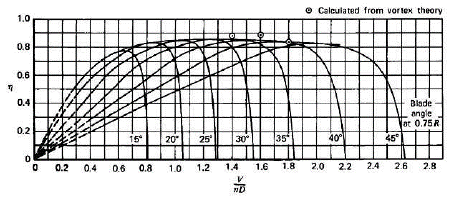
\includegraphics{images/part7/advanceratioeffi.png}
    \caption{Typical propeller efficiency curves as a function of advance ratio $J$ \cite{bronz2012multi}.}
    \label{fig:advratioeffi}
\end{figure}

\begin{equation}
    J = \frac{Z}{n D_p}
    \label{eq:advratio}
\end{equation}

Substituting the following definitions of the relative wind speed $Z$ and the rotational speed of the propeller $n$ which are specific to this case, one obtains Equation \ref{eq:advanceratiodw}, where $R_w$ is the radius of the wheels and $i$ the gear ratio.

\begin{equation}
    Z = V-W
    \label{eq:relativevel}
\end{equation}

\begin{equation}
    n = \frac{i V}{R_w}
    \label{eq:rpm}
\end{equation}

\begin{equation}
    J = \frac{V-W}{i V D_p}R_w
    \label{eq:advanceratiodw}
\end{equation}

Equation \ref{eq:advanceratiodw} illustrates that the advance ratio is not constant over the operational domain. This is also shown on Figure \ref{fig:advanceratios}. The advance ratio for this case is plotted for various gear ratios. Possessing the ability to vary the pitch of the propeller is therefore of great help in maximising the efficiency of the propeller and achieving the best results possible.

\begin{figure}
    \centering
    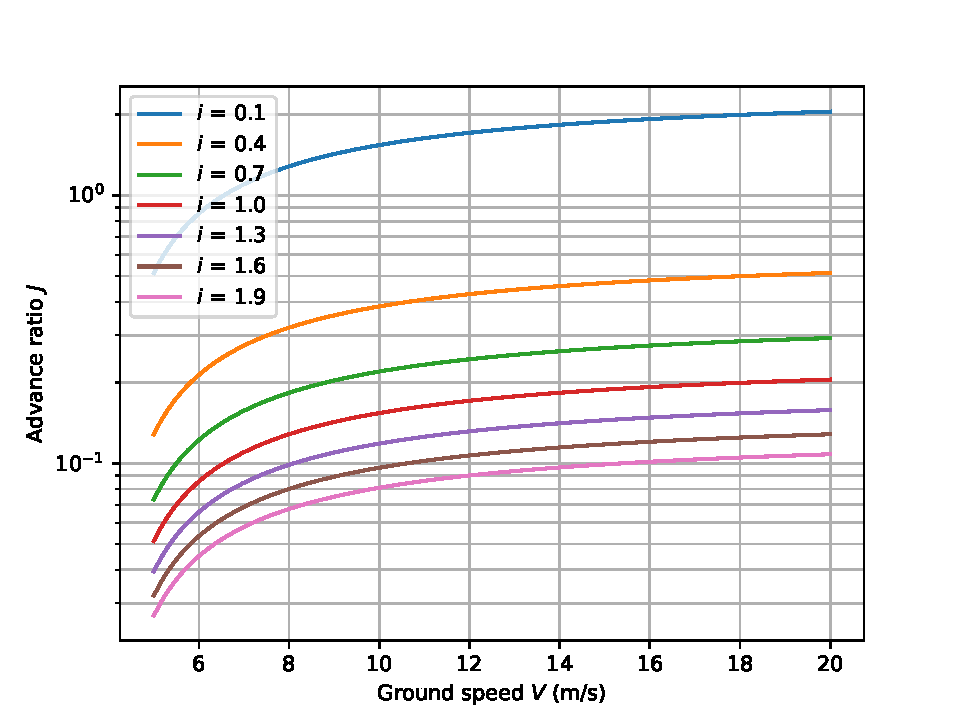
\includegraphics[width = 0.7\linewidth]{images/part7/advance ratios.pdf}
    \caption{Advance ratio as a function of ground speed. $i$ is the gear ratio. Values of $D_p$ and $R_w$ taken from the final design values. An arbitrary wind speed of $4\mathbf{m.s}^{-1}$ was taken.}
    \label{fig:advanceratios}
\end{figure}

The aim is to change the pitch angle of all propeller blades by the same amount, reliably, precisely, and easily so that it can be performed during the wind tunnel experiments without the risk of producing unbalanced thrust. The blades would need at least a pitch angle range of 30 degrees for it to be impactful.

The hub needed to fit and attach securely onto a 16mm diameter propeller shaft chosen due to its high polar moment of inertia, resulting in good torsional strength. It would be expected to spin at around 600 RPM, hence support the high centrifugal forces of the propeller blades, but also unscrew reasonably easy to change the configuration if needed.

\subsection{Design process}

Initially, a swash-plate mechanism similar to those seen on helicopters was studied. It simultaneously changes all blade angles. A motor would be used to slide a plate up and down to control the blade angle even whilst testing the vehicle in the wind tunnel. However, its intricacy was deemed too high for the design requirements set. Figure \ref{fig:swash} shows the initial design. Hence a simpler revision was created. Each blade was to be rotated individually and manually. Being a structurally important component, the hub was built in aluminium and stainless steel to be able to withstand far greater stresses than it would experience in testing. This also meant that the hub could be reusable for larger scale vehicle designs.

\begin{figure}[!htbp]
    \centering
    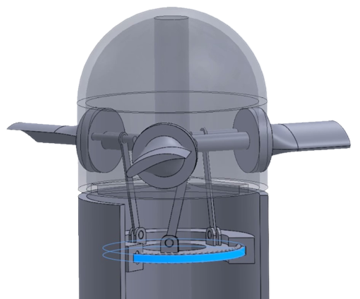
\includegraphics{images/part7/swash.png}
    \caption{Initial swash-plate-like hub design}
    \label{fig:swash}
\end{figure}

The first design iteration of the hub is shown in Figure \ref{fig:iter2}. It utilises a circular shape to fit the blades around the hub. An aluminium blade root is attached to the blade with three bolts, inserted in the main part of the hub, and can therefore be rotated for each blade, enabling a range of pitch angles of 30 degrees. This design could be modified easily to fit three blades as well. However, because of the circular shape of the faces connected to the blades, the overall diameter of the hub was too wide. Since the propeller diameter is constrained, it is important to minimize the size of the hub so that the blades can be longer and produce more thrust.

\begin{figure}[!htbp]
    \centering
    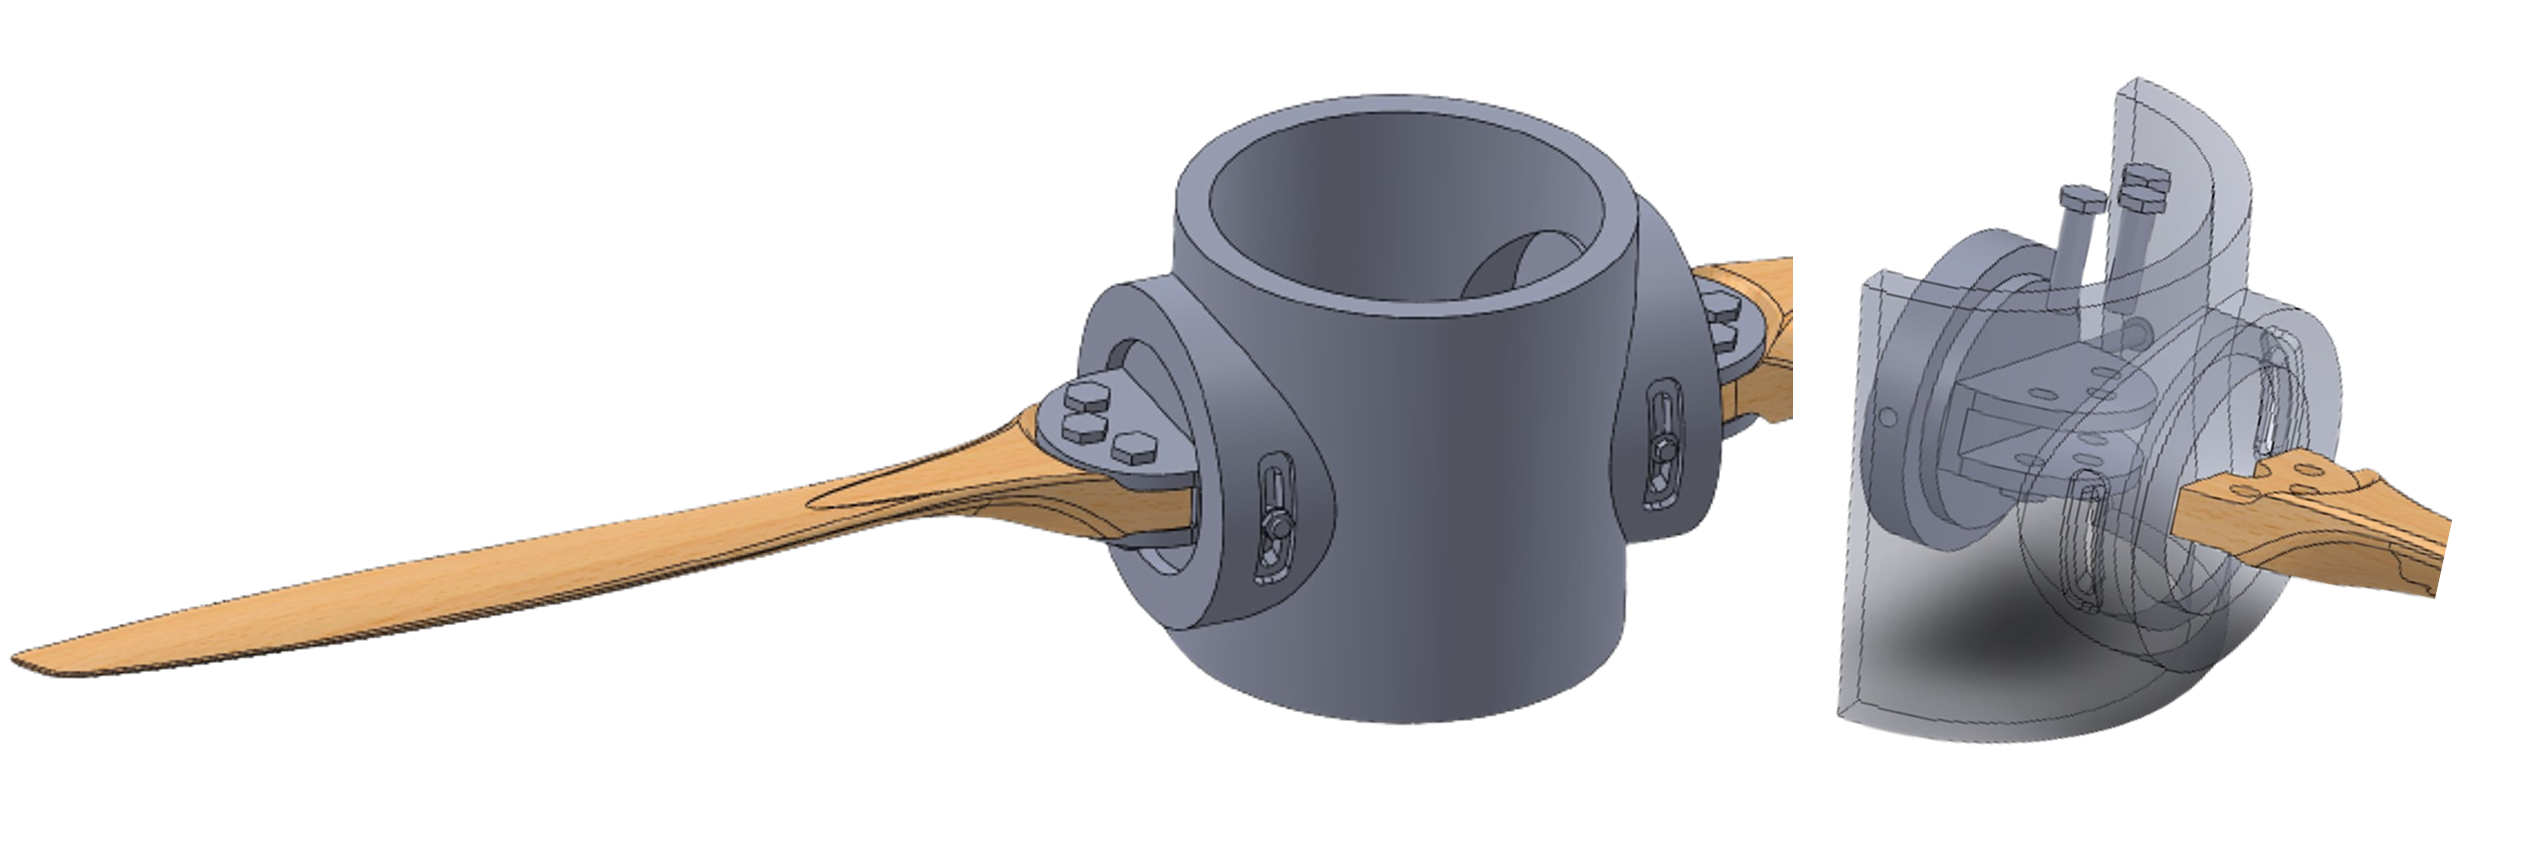
\includegraphics[width=\linewidth]{images/part7/iter2.png}
    \caption{Dual-blade circular hub design}
    \label{fig:iter2}
\end{figure}

\begin{figure}[!htbp]
    \centering
    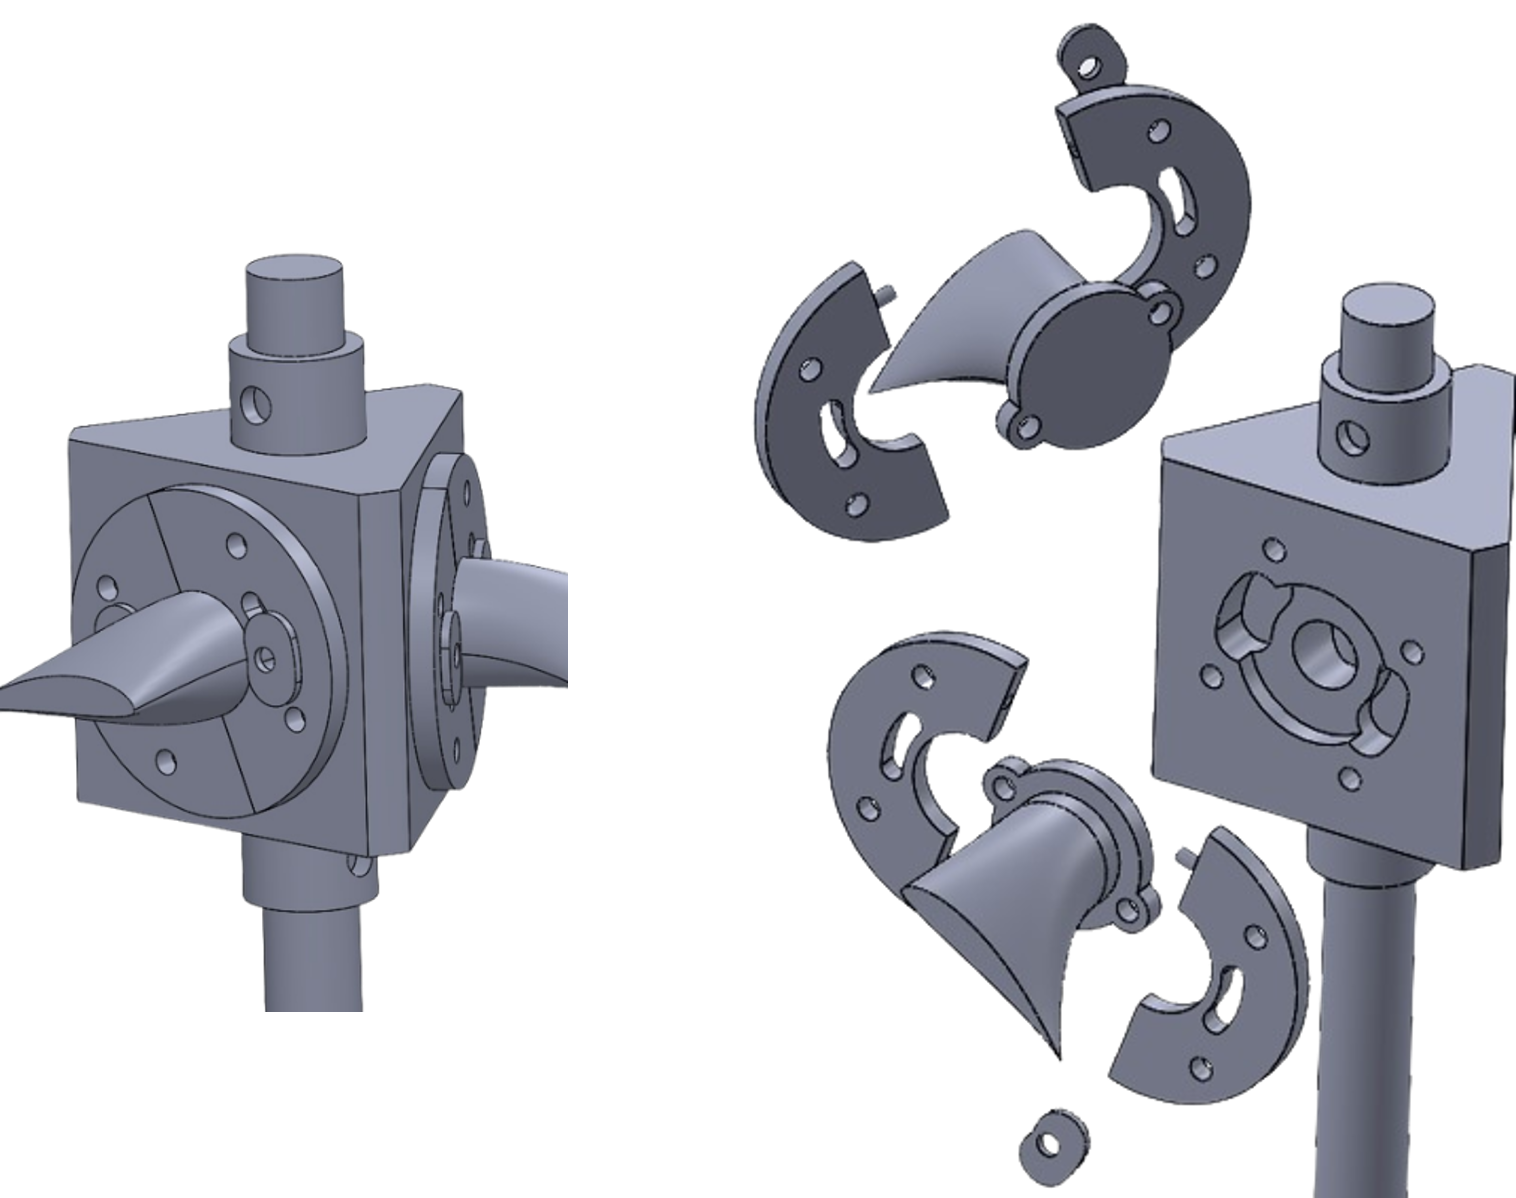
\includegraphics{images/part7/explodedhub.png}
    \caption{Collapsed and exploded view of the final hub design}
    \label{fig:explodedview}
\end{figure}

Therefore, for the second iteration shown in Figure \ref{fig:explodedview}, the shape was more triangular. With the faces on which the blades fix onto the hub being flat, this reduces the amount of excess material used and reduces the overall diameter of the hub. The diameter of the hub is only 71 mm. It consists of more separate pieces as can be seen on the exploded view in Figure \ref{fig:explodedview}, but is a lot more compact.

\subsection{Manufacturing}

Being a structurally important component, the hub was built in aluminium. The propeller can be reasonably expected to be able to spin at 600 RPM and withstand the necessary centrifugal forces of the blades, which has been estimated to be around 5.3 N per blade.

The hub was made by the EDMC and had to be designed to simplify the machining process, reducing the manufacturing cost of the part. The parts securing the blades to the hub were cut from a sheet of aluminium using a water-jet cutter.

\begin{figure}[tbp]
    \centering
    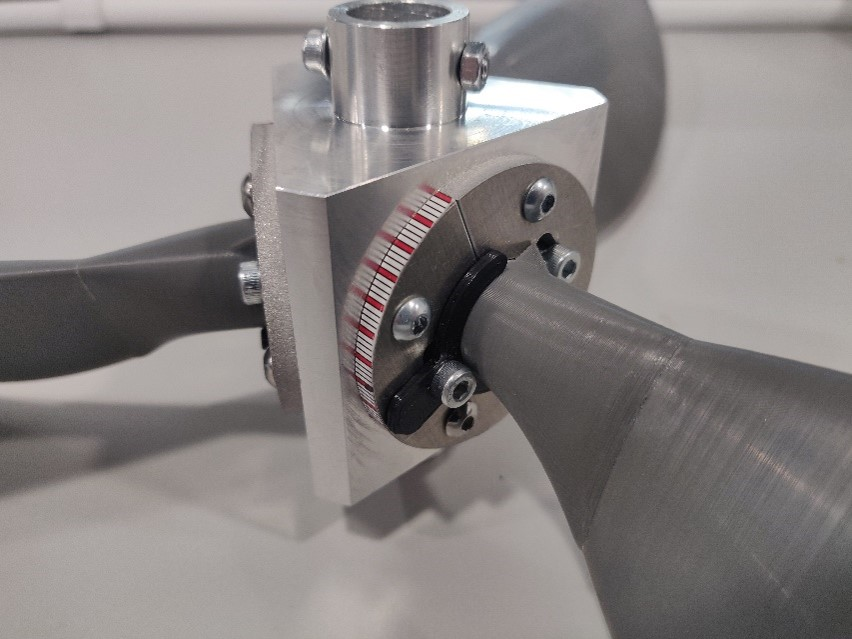
\includegraphics{images/part7/finalphoto.jpg}
    \caption{Final manufactured hub}
    \label{fig:finalhub}
\end{figure}
